
\documentclass[runningheads]{llncs}
\usepackage{graphicx}
\usepackage{hyperref}
\usepackage{csquotes}
\usepackage{array}
\usepackage{textcomp}
\newcolumntype{x}[1]{>{\centering\arraybackslash\hspace{0pt}}p{#1}}

\begin{document}
	
	\title{Explain variable influence in black-box models through pattern mining}
	\titlerunning{Master Thesis Proposal}
	\author{Xiaoqi Ma}
	\institute{RWTH Aachen University \\
		\email{xiaoqi.ma@rwth-aachen.de}\\}
	\maketitle  
	
	\begin{abstract}
		
		Understanding the decisions made by machine learning models is crucial for decision-makers and end-users. Enforced by GDPR, "right to explanation" demands businesses to provide understandable justifications to their users. Thus, it is of paramount importance to elucidate the model decision, which could be measured by model interpretability, the degree to which a human can understand the cause of a decision. In order to interpret black-box models, model-agnostic approaches could be applied, which provide flexibility in the choice of models, explanations and representation for models. From global interpretability viewpoint, feature importance and global surrogate are going to be explored. We also investigate the local model-agnostic methods, like LIME and Shapley value. After obtaining the designated feature contribution for each instance, we could use the subgroup discovery technique to figure out "interesting" patterns to provide more elaborate explanations. In this thesis, the aim is to build up a python package to provide a collection of tools to explain variable influence in black-box models through subgroup discovery. 
		
		\keywords{Black-box model  interpretability \and Model-agnostic  \and Subgroup discovery}
	\end{abstract}

	\section{Introduction}
	
	Machine learning is a set of methods that are used to teach computers to perform different tasks without hard-coding instructions. Over the last decades, Machine learning area has gone through unprecedented growth. Due to the increasing computational power, a myriad of classification or regression tasks could be solved by applying machine learning algorithms. For a simple classification task, like predicting the house prices based on the historical data, a traditional regression model is adequate, like logistic regression. However, for tackling complex problems like language translation, more complicated models are required, such as neural networks. 
	
	When evaluating machine learning models, people have a tendency to focus on the performance by observing metrics like accuracy, precision, recall and etc., which are of course very fundamental. Nevertheless, they neglect the importance of interpretability for the model, which shows the degree for a human can consistently predict the model\textquotesingle s result\cite{kim2016examples}. As Albert Einstein once said, "If you can\textquotesingle t explain it simply, you don\textquotesingle t understand it well enough". Therefore, to have a better understanding of the decisions made by the model, it is of paramount importance to achieve high model interpretability.
	
	For those models that can be easily explained are called \textit{Interpretable models}, such as linear regression, logistic regression, and decision trees, since the prediction results could be interpreted by exploring into the model parameters. On the contrary, ensemble models or neural networks could be regarded as \textit{Black-box models} that decisions cannot be understood by looking at their parameters, which is a major disadvantage for complex models. Typically, those complicated models could achieve better performance while provides less interpretability. However, proper interpretability is crucial to explain the choice made by the model and especially important for decision-makers. Besides, "right to explanation" meaning the right to be given an explanation for an algorithm\textquotesingle s output was stated by General Data Protection Regulation(GDPR), which requires businesses to provide understandable justifications to their users \cite{voigt2017eu}.
	
	To understand model predictions, some explanation methods are necessary, which are algorithms to provides explanations. An explanation usually links the input feature values of an instance to its model prediction in a human understandable way \cite{molnar2019}. There are plenty of properties of explanation methods, and one of them is the \textit{Degree of Importance}, which reflects the importance of features in the explanation\cite{robnik2018perturbation}. Several approaches calculating the feature importance score are available, and we could rank the score to obtain a general overview of the most dominating features in the black-box model. According to the contributions of the specific variable, we might go step further to find out more detailed explanations through subgroup discovery technique, which is a data mining technique to automatically discover similar patterns from dataset. For example, once we know the education level is a supreme feature in predicting the salary, we might want to dig some patterns that comply with this prediction or even disagree with this prediction.  
	
	Thus, this thesis is aimed to explain the effect of independent variables with the help of pattern mining technique to facilitate understanding decisions.
	
	
	\section{Related Work}
	
	When taking a closer look at the properties of explanation methods stated in \cite{robnik2018perturbation}, the property that “degree of importance” which reveals the importance of the feature in an individual instance might be interested to investigate. The permutation feature importance measurement was first introduced by Breiman for random forests \cite{breiman2001random}. Then, one of the variants called model reliance was proposed in \cite{fisher2018model}. 
	
	Recently, model-agnostic approaches for explaining black-box are being developed. In \cite{ribeiro2016should}, a novel explanation technique, called LIME,  that explains the predictions of any classifier in an interpretable and faithful manner by learning the instances locally was introduced. Additionally, a unified framework for predictions interpretation was proposed, know as SHAP (SHapley Additive exPlanations). For every instance prediction, each feature was assigned an importance value to represent the contribution for the prediction \cite{lundberg2017unified}.
	
	Back in 2008, an exceptional model mining, which is used to discover subgroups with a model over multiple attributes as target concept, was first introduced in \cite{leman2008exceptional}. Leman et al. also presented a variety of model classes and discussed appropriate interestingness measures, including the correlation model. The correlation model was aimed to measure the dependence between the two numeric attributes utilizing the well-known correlation coefficient measurement, which is one of the models that would be seelcted to mine subgroups in this thesis. 
	
	We have seen many papers presenting various methods to provide model explanations, however, to the best of our knowledge, there is no work addressing the black-box model explanation through subgroup discovery technique. Thus, we are excited to find out some interesting results for explaining black-box models through pattern mining. 
	
	\section{Research questions}
	
	The following research questions shall be covered in this thesis. 
	
	\begin{enumerate}
		\item How can we identify the importance of a specific variable in a black-box model?
		\item How can we discover interesting subgroups under consideration that we constrain on specific variables?
		\item How can we avoid the redundancy in discovered subgroups? And how can we stabilize the results?
		\item How can we make sure the explanation is desirable and reliable?
	\end{enumerate}
	
	To comprehend and interpret the whole model, we need \textit{global interpretability}, which means we can understand and explain the interactions between dependent variables and independent variables based on the complete dataset. Trying to figure out the feature importance is always a good step to have a good grasp of global interpretability. Nevertheless, the interactions between input features might have an impact on the analysis, like the existence of collinear variables in the same model, which has to be taken into account.
	
	After global interpretability exploration, we might be interested to understand "Why did the model make specific decisions for a single instance?", which leads to \textit{local interpretations}. In this case, we focus on each instance and try to understand the model decision for this specific instance based on this local region. Furthermore, we could discover subgroups of the dataset with statistically interesting decisions \cite{wrobel2001inductive}. In this thesis, we would adopt the \textit{Exceptional model mining} framework to mine subgroups \cite{leman2008exceptional}. Obviously, we would like to avoid redundancy in those subgroups, therefore, the choice of quality measures is of big concern. Another issue is the stability of our model interpretation, which requires further discussion in this thesis. Last but not least, the explanations are supposed to be trustworthy and meaningful. 
	
	\section{Methods}
	
	\subsection{Model-agnostic methods}
	
	Apart from the \textit{model-specific} methods which are intrinsically interpretable, \textit{model-agnostic} methods can be applied on any machine learning model, which provides a generic framework for interpretability that allows for flexibility in the choice of models. Desirable aspects of a model-agnostic explanation system are model flexibility, explanation flexibility, and representation flexibility as stated in \cite{ribeiro2016model}. The following approaches which belong to model-agnostic methods will be potentially practiced to provide better explanations for model decisions. 
	
	\subsubsection{Feature importance}
	The feature importance is measured by the increase in the prediction error of the model after permuting the feature, which is known as permutation importance measurement. A feature is regarded as "important" if prediction error increases after shuffling feature values as the model depends on the feature for the prediction. Conversely, a feature is "unimportant" if prediction error seldom changes, which means the feature is hardly relied on for the model. Based on this idea, Fisher, Rudin, and Dominici proposed a model-agnostic version of the feature importance and called it model reliance \cite{fisher2018model}.
	
	\subsubsection{Local Surrogate}
	To explain individual predictions of black box machine learning models, local surrogate model is a good choice. Instead of approximating the predictions of the underlying black box model like global surrogate models, the local surrogate model focuses on explaining predictions for an individual instance. Local interpretable model-agnostic explanations (LIME), a well-received implementation for the local surrogate, provides human-friendly interpretation and is currently available for application usage. The python package is accessible in \cite{lime}, and they claim to support explaining individual predictions for tabular data, texts, and images.
	
	\subsubsection{Shapley values }
	The Shapley value, coined by Shapley, is a method for assigning payouts to players depending on their contribution to the total payout. Players cooperate in a coalition and receive a certain profit from this cooperation \cite{shapley1953value}. It can also be used as a locally accurate additive feature attribution method, and in this case, the shapley value is the average contribution of a feature value across all possible coalitions.
	
	\subsection{Subgroup discovery methods}
	
	A subgroup discovery task is specified by a quadruple (D, $\Sigma$, T, Q). D is a dataset. $\Sigma$ defines the search space of candidate subgroup descriptions in this dataset. The target concept T specifies the property of interest for this discovery task. Finally, Q defines a set of selection criteria that depends on the target concept. Among them, the target concept is of vital importance, therefore, the following two scenarios might be discussed in detail.
	
	\subsection{Numeric target }
	
	Since we obtain the particular feature importance or contribution for each instance from the previously mentioned methods, which determines that the target value is numeric. For handling numeric attributes, one possible way is to convert numeric values to binary target values, which are more suitable for subgroup discovery task. Nevertheless, numeric discretization might fail to show the complete distribution of numeric attributes, which may lead to confusing results. Thus, another feasible approach is to compare the subgroup description of the target with respect to the distributional properties in the whole dataset, e.g. the mean value, the median value, or the variance of the target.
	
	\subsection{Complex target }
	
	In this case, the property of interest is not specified by a single attribute, but by a set of attributes, and subgroups can be discovered by a variant of subgroup discovery technique called \textit{exceptional model mining}. The goal of exceptional model mining is to identify subgroup descriptions, for which the model parameters differ significantly from the parameters of the model built from the entire dataset \cite{leman2008exceptional}. A simple example of a model class is the correlation model. e.g. the Pearson correlation between the feature value change and the corresponding prediction change. By observing the extraordinary strong correlation between two numeric attributes, we could identify desired subgroups. 
	
	\section{Initial Experiments}
	
	We will work on a real-world dataset about Census income, also known as the Adult dataset available in the UCI ML Repository, where we will predict if the potential income of people is more than \$50K/year or not.
	
	As declared before, one way to explain model predictions is to examine the permutation importance of the features. Typically, ELI5\cite{eli5} provides weights along with bias for each feature demonstrating how influential it might have been in contributing to the final predictions across the entire dataset. As presented in Figure \ref{fig:feature_weights}, the first column means feature weights and bias, and the second column shows the feature name. It is evident those top ranking features are of crucial effect in this dataset, such as capital gain, education-num and age. Then, we might want to investigate feature importance for individual instance, which is fortunately also supported by the library. As shown in Figure \ref{fig:individual_importance}, the first column shows the contribution weights each feature has, and the next two columns represent feature names and corresponding feature values. As seen from the label, this person earns more than \$50K/year, which is highly credited with his high education level and stable relationship.
	
	\begin{figure}
		\centering
		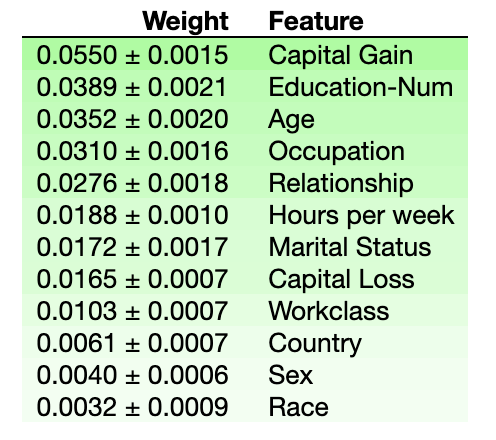
\includegraphics[width=0.6\textwidth]{img/feature_weights.png}
		\caption{Feature importance weights for entire dataset}
		\label{fig:feature_weights}
	\end{figure}

	\begin{figure}
		\centering
		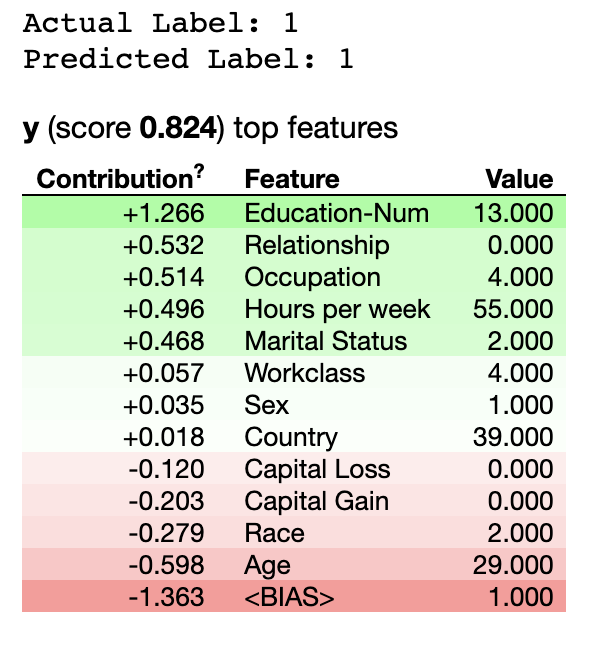
\includegraphics[width=0.6\textwidth]{img/individual_importance.png}
		\caption{Feature importance weights for a single instance}
		\label{fig:individual_importance}
	\end{figure}
	
	Another interesting experiment was done through SHAP library\cite{lundberg2017unified}, offering a unified approach to explain the output of any machine learning model. SHAP is typically used to explain decisions for an individual instance, by assigning each feature an importance value for a particular prediction. As depicted in Figure \ref{fig:shap}, SHAP gives nice reasoning below showing which features are the most influential in the model taking the correct decision of predicting the person\textquotesingle s income. The below explanation shows features each contributing to push the model output from the base value (the average model output over the training dataset we passed) to the actual model output. Features pushing the prediction higher are shown in red, those pushing the prediction lower are in blue. It is obvious to notice that education-num, relationship and occupation dominate the prediction to some degree. 
	
	\begin{figure}
		\centering
		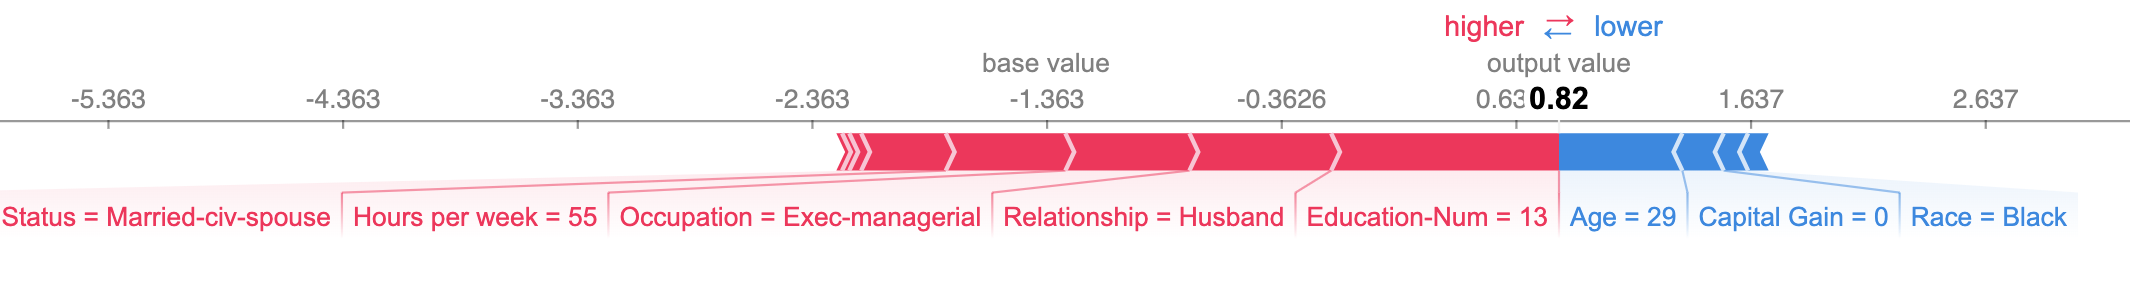
\includegraphics[width=1.2\textwidth]{img/shap.png}
		\caption{SHAP value for each feature of a single instance}
		\label{fig:shap}
	\end{figure}
	
	Additionally, we could use the dependence plot to show the effect of a single feature across the whole dataset. They plot feature\textquotesingle s values vs. the SHAP value of that feature across instances. As plotted in Figure \ref{fig:edu_dependence}, the vertical axis represents SHAP value for education-num, and the horizontal axis indicates the feature values of education-num. Actually, another feature could be chosen for coloring dots to show feature interactions, however, for simplicity, the dependent feature is set as education-num as well. From the plot, it is noticed that the SHAP value climbs with the increment of education-num, which means higher education level generally contributes more for the prediction.
	
	\begin{figure}
		\centering
		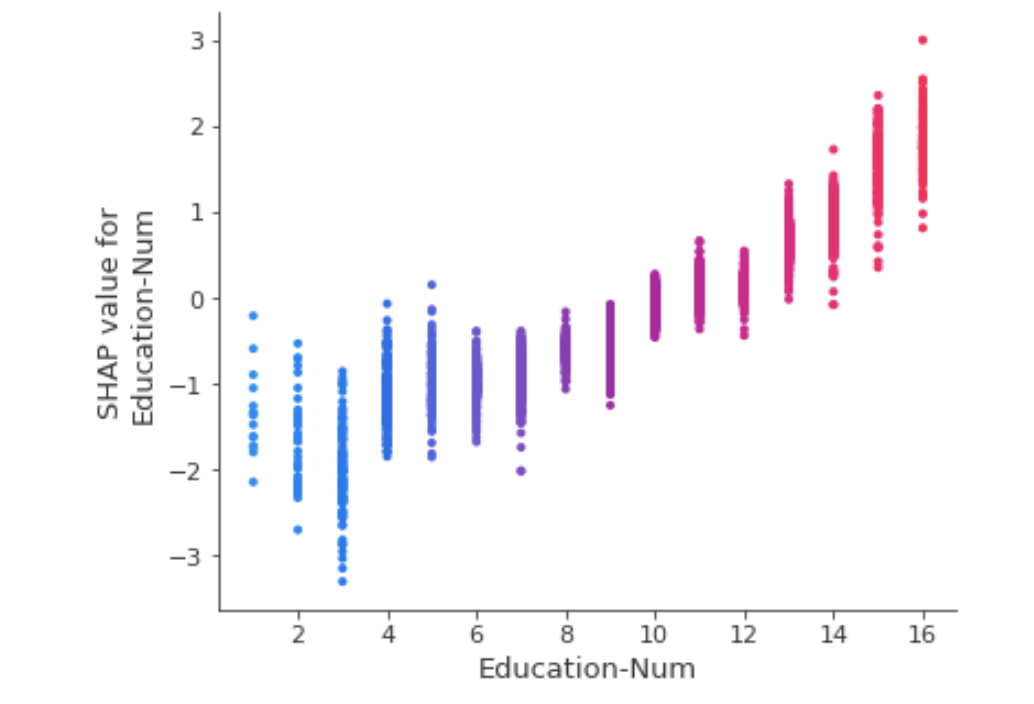
\includegraphics[width=1.0\textwidth]{img/education_dependence_plot.png}
		\caption{SHAP dependence plot for education-num}
		\label{fig:edu_dependence}
	\end{figure}

    Furthermore, treating the SHAP value of education-num as numeric target concept, subgroups could be discovered by the pysubgroup library \cite{lemmerich2018pysubgroup}. As seen from Figure \ref{fig:edu_sg_discovery}, we could conclude that people work as Prof-specialty have a stronger tendency to earn more than 50K\$/year. Nevertheless, those subgroup descriptions are pretty similar, which requires further methods to reduce redundancy. In addition, optimized quality measurement shall be developed for the next step.

	\begin{figure}
		\centering
		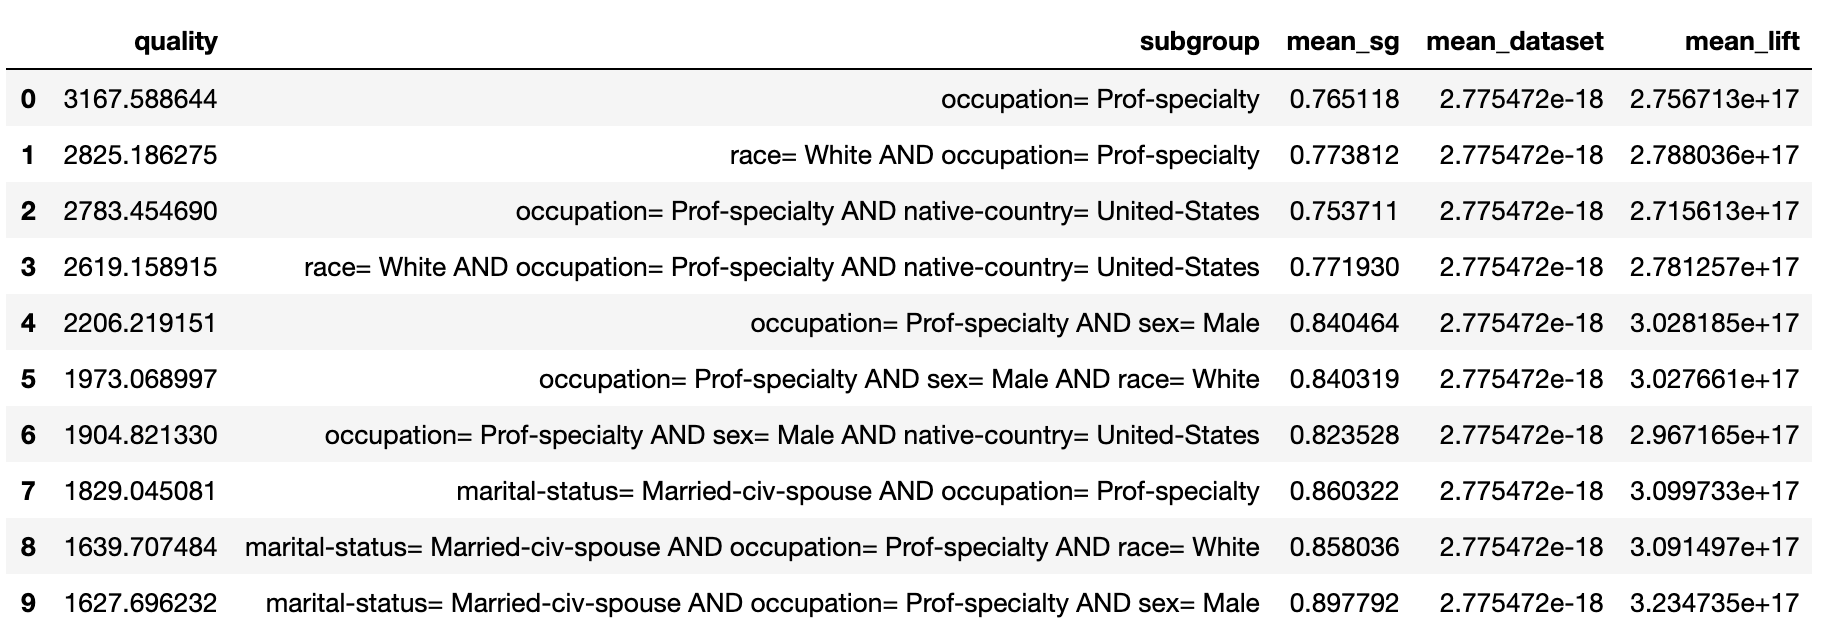
\includegraphics[width=1.2\textwidth]{img/edu_sg_discovery.png}
		\caption{Subgroup discovery result with SHAP value of education-num as target}
		\label{fig:edu_sg_discovery}
	\end{figure}

	\section{Possible obstacles}
	
    First, from global interpretability perspective, we need to calculate the importance for each future. Meanwhile, we need to figure out an elegant method to cope with collinear variables. Besides, the interactions between input features should be considered as well. Through an initial experiment, we know that not all algorithms are suitable for mixed-type tabular data, which contains numeric and categorical features. Therefore, it deserves discussion about whether we modify categorical data by either label encoding or one-hot encoding or adjust numerical data by discretization. What\textquotesingle s more, while using subgroup discovery techniques, the choice of quality measurement plays a vital role. Moreover, we not only need to keep an eye on the algorithm performance but also value stability and reliability. Even though more challenges might have emerged, we believe all obstacles shall be solved. 

	\section{Potential achievement}
	
	The aim is to build up a python package to provide a collection of tools to explain variable influence in black-box models through subgroup discovery. Ideally, it should at least support the following functions:
	
	\begin{enumerate}
		\item Provide data preprocessing methods, including feature encoding, data cleaning and etc.
		\item Calculate the feature importance score using various methods
		\item Identify the feature contribution for a single instance
		\item Discover subgroups relying on the feature importance/contribution
		\item Visualize results in an elegant way
	\end{enumerate}
	
	\section{Time Schedule for Master’s Thesis }
	
	\begin{table}
		\centering
%		\caption{Visual features based related work }
		\begin{tabular}{| l | c | }
			\hline
			Task Completed & Due data\\
			\hline
			Topic Approved & 01-06-2019  \\
			Preliminary literature review & 15-06-2019 (2 weeks) \\
			Initial Implementation and experiment & 29-06-2019 (2 weeks) \\
			Prepare datasets & 06-07-2019  (1 week) \\
			Improve implementations & 27-07-2019 (3 weeks) \\
			Conduct experiment & 10-08-2019 (2 weeks) \\
			Implement extensions/variations & 31-08-2019 (3 weeks) \\
			Conduct more experiment & 14-09-2019 (2 weeks) \\
			Writing thesis draft & 26-10-2019 (6 weeks) \\
			Revise thesis draft & 16-11-2019 (3 weeks) \\
			Final thesis draft submission & 30-11-2019 (2 weeks) \\
			\hline
		\end{tabular}
		
	\end{table}
	
	

	% prevents nocite errors
	%	\nocite{*}
	\newpage
	\bibliography{literature}
	\bibliographystyle{IEEEtran}
	
	
\end{document}